\documentclass[psamsfonts]{amsart}

%-------Packages---------
\usepackage{amssymb,amsfonts}
\usepackage[all,arc]{xy}
\usepackage{enumerate}
\usepackage[margin=1in]{geometry}
\usepackage{amsthm}
\usepackage{theorem}
\usepackage{verbatim}
\usepackage{tikz}
\usepackage{hyperref}
\usetikzlibrary{shapes,arrows}

\newenvironment{sol}{{\bfseries Solution:}}{\qedsymbol}
\newenvironment{prob}{{\bfseries Problem:}}

\bibliographystyle{plain}

\voffset = -10pt
\headheight = 0pt
\topmargin = -20pt
\textheight = 690pt

%--------Meta Data: Fill in your info------
\title{14.27 \\
Economics of E-Commerce \\
Problem Set 2}

\author{John Wang}

\begin{document}

\maketitle

\section{Problem 4}

\begin{prob}
Spend a few minutes on Google Trends exploring anything your heart contents to get warmed up. Then think of a few online companies that compete with one another and compare them using both the searches and the website features. What can you infer from the data? Can you find any interesting or surprising results?
\end{prob}
\begin{sol}
I examined the trends of Amazon.com and eBay.com. Both of these companies are similar, in that they can be categorized in the online marketing and retail industry, but they differ by the types of products they sell. For instance, eBay is more of a second hand auction site, although it is moving towards an online retail business, while Amazon has much more retail business, especially in brand name products. This distinction can provide some insight into their different Google trends.

\begin{figure}[h!]
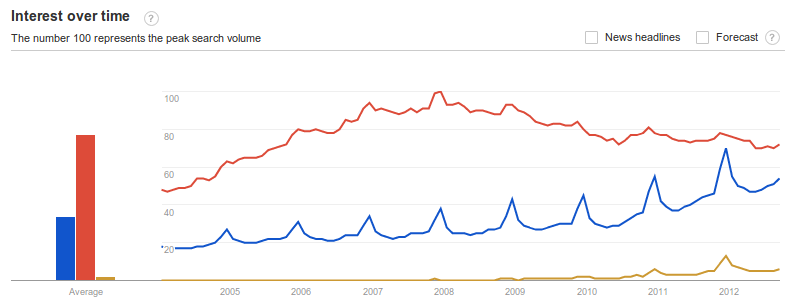
\includegraphics[width=6in]{ebay_vs_amazon.png}
\caption{eBay (Red Line) vs Amazon (Blue Line) on Google Trends}
\end{figure}

It is clear from the figure above that Amazon and eBay have completely different trends on Google searches. First, we can see that eBay seems to have reached some sort of saturation point for its growth in Google searches, whereas Amazon currently has an upward trend which is moving higher every year. This could be a reflection of the different growth phases which each company is currently in, since eBay already controls a large part of the online auction market and has few innovative products for expansion, whereas Amazon has many new technologies each year, and is pushing hard for new users. 

The other trend to notice is that Amazon is highly cyclical, depending on the season, whereas eBay is not. For Amazon, sales spike up without fail every December (probably due to the Christmas and Holiday season when gifts are prevalent). Ebay, however, does not perceptibly seem to be affected by seasonality. This could come from the fact that Amazon and eBay have different lines of business. In Amazon's more retail centered business, consumers usually purchase new, front-line items which were just released. Since Amazon provides a online platform for businesses to sell their latest products, consumers on Amazon are more likely to purchase gifts. However, eBay targets a set of suppliers which have an older domain of items. These are usually second hand or outdated products, which are less likely to be given as gifts. Thus, eBay sees much less of a seasonal trend, and Google searches for eBay grow much more organically.


\end{sol}

\end{document}
